\def\thelstlisting{}

%不需要区分奇偶页的请使用下面一行
\documentclass[a4paper,AutoFakeBold,oneside,12pt]{book}
%需要区分奇偶页的(即每一章第一页一定在奇数页上)请使用下面一行
%\documentclass[a4paper,AutoFakeBold,openright,12pt]{book}
\usepackage{BUPTthesisbachelor}
\usepackage{setspace}

%\lstdefinestyle{sharpc}{language=[Sharp]C, frame=lrtb, rulecolor=\color{blue!80!black}}


%%%%%%%%%%%%%%%%%%%%%%%%% Begin Documents %%%%%%%%%%%%%%%%%%%%%%%%%%
\begin{document}

% 封面
\blankmatter

\includepdf[pages=-]{docs/cover.pdf}

% 任务书
\blankmatter

\includepdf[pages=-]{docs/task.pdf}

% 成绩评定表
\blankmatter

\includepdf[pages=-]{docs/scoreTable.pdf}

% 诚信声明
\blankmatter

\includepdf[pages=-]{docs/statement.pdf}

%%%%%%%%%%%%%%%%%%%%%%%%%%%%%%%%%%%%%%%%%%%%%%%%%%%%%%%%%%%%%%%%%%%%
%                                                                  %
%   Copyright (c) 2010 - 2011 Caspar Zhang <casparant@gmail.com>   %
%                                                                  %
%   This copyrighted material is made available to anyone wishing  %
%   to use, modify, copy, or redistribute it subject to the terms  %
%   and conditions of the GNU General Public License version 2.    %
%                                                                  %
%   This program is distributed in the hope that it will be        %
%   useful, but WITHOUT ANY WARRANTY; without even the implied     %
%   warranty of MERCHANTABILITY or FITNESS FOR A PARTICULAR        %
%   PURPOSE. See the GNU General Public License for more details.  %
%                                                                  %
%   You should have received a copy of the GNU General Public      %
%   License along with this program; if not, write to the Free     %
%   Software Foundation, Inc., 51 Franklin Street, Fifth Floor,    %
%   Boston, MA 02110-1301, USA.                                    %
%                                                                  %
%%%%%%%%%%%%%%%%%%%%%%%%%%%%%%%%%%%%%%%%%%%%%%%%%%%%%%%%%%%%%%%%%%%%

% 你只需要修改下面几行就可以完成大部分内容的填写,
% 这要求你具有一定的LaTeX基础,但是如果你足够聪明,
% 不具有LaTeX基础也可以完成。

% 论文中文题目
\def\thesistitle{基于知识图谱的可视化系统的设计与实现}

% 论文英文题目
%提示:英文摘要页的标题注意格式要求。
\def\thesistitleen{Design and Implementation of Visualization System Based on Vulnerability Knowledge Graph}

% Thank Words
\def\thankwords{

感谢。

}
    % Main items 
%%%%%%%%%%%%%%%%%%%%%%%%%%%%%%%%%%%%%%%%%%%%%%%%%%%%%%%%%%%%%%%%%%%%
%                                                                  %
%   Copyright (c) 2010 - 2011 Caspar Zhang <casparant@gmail.com>   %
%                                                                  %
%   This copyrighted material is made available to anyone wishing  %
%   to use, modify, copy, or redistribute it subject to the terms  %
%   and conditions of the GNU General Public License version 2.    %
%                                                                  %
%   This program is distributed in the hope that it will be        %
%   useful, but WITHOUT ANY WARRANTY; without even the implied     %
%   warranty of MERCHANTABILITY or FITNESS FOR A PARTICULAR        %
%   PURPOSE. See the GNU General Public License for more details.  %
%                                                                  %
%   You should have received a copy of the GNU General Public      %
%   License along with this program; if not, write to the Free     %
%   Software Foundation, Inc., 51 Franklin Street, Fifth Floor,    %
%   Boston, MA 02110-1301, USA.                                    %
%                                                                  %
%%%%%%%%%%%%%%%%%%%%%%%%%%%%%%%%%%%%%%%%%%%%%%%%%%%%%%%%%%%%%%%%%%%%

% 你只需要修改下面内容就可以完成中英文摘要,
% 这要求你具有一定的LaTeX基础,但是还是那句话,
% 如果你足够聪明,不具有LaTeX基础也可以完成。

% 中文摘要
\def\abstractzh{
%从这里开始写你的摘要,分段需要空一行。
这是中文摘要的部分。

它可以拥有多段。
这是中文摘要的部分。

它可以拥有多段。

如果你写的太长,甚至可以到第二页。
%摘要结束
}

% 中文关键字 
% TODO: 改成可变长度的
\def\abszhkeyone{北京邮电大学}
\def\abszhkeytwo{本科生}
\def\abszhkeythree{毕业设计}
\def\abszhkeyfour{模板}
\def\abszhkeyfive{示例}

% ABSTRACT
\def\abstracten{
%Your abstract here, to make a new paragraph, give an extra blank line please.
This is ABSTRACT.

You can write more than one paragraph here.

If your abstract is too long, it will take up more pages. 
%Abstract done
}

% Key Words 
% TODO: 改成可变长度的
\def\absenkeyone{BUPT}
\def\absenkeytwo{undergraduate}
\def\absenkeythree{thesis}
\def\absenkeyfour{template}
\def\absenkeyfive{example}


  % Abstract
\fancypagestyle{plain}{\pagestyle{frontmatter}}
\frontmatter\tableofcontents % Content


% 正文
\newpage\mainmatter
\fancypagestyle{plain}{\pagestyle{mainmatter}}
%\let\cleardoublepagebak=\cleardoublepage
%\let\cleardoublepage\relax % Make new chapter stay on old page

%%%%%%%%%%%%%%%%%%%%%%%%%%%%% Main Area %%%%%%%%%%%%%%%%%%%%%%%%%%%%

\chapter{绪论}

\section{项目背景及意义}

\subsection{选题背景}
% 这段先放着
% \begin{definition}
% 	计算机安全、互联网信息安全,或信息安全技术意指对计算机系统及计算机网络施加保护手段,以使其不受信息披露、信息盗取、软硬件或电子信息损坏等危害,使其\cite{wilson_fundamental_2014}
% \end{definition}
% 这段先放着

近年来,随着互联网产业迅速发展,互联网安全漏洞问题的显著性也急剧增加。公共漏洞和暴露(Common Vulnerabilities and Exposures, CVE)等权威漏洞数据档案库的数据显示,自 1999 年该漏洞库库首次披露安全漏洞以来,互联网安全漏洞年新增数量呈增长趋势。2019 年全年,新增漏洞两万余个;2020 年全年新增漏洞三万五千余个。随着现代软件系统复杂度提升、互联网加速漏洞信息传播,对攻击者而言,不仅漏洞攻击的学习成本和实施难度下降,其可以利用的漏洞数量也明显增多;对企业与开发者而言,随着开源化逐渐成为一种潮流趋势,各类计算机软硬件与互联网产品对开源项目的依赖性随之提高。正如近期 Java Log4j 日志组件漏洞造成全球互联网范围的大规模信息安全问题,计算机与互联网产业蓬勃发展的同时,也面临与日俱增的信息安全挑战。

\subsection{项目意义}

本课题针对上述问题,提出一种漏洞知识图谱可视化系统。基于爬虫抽取、知识图谱、图数据库、可视化前端等技术,对多种数据源的互联网公开漏洞数据,包括漏洞描述及风险评估、受影响资产、可利用代码及补丁等信息进行收集与分析,通过对异构数据源抽取的数据进行实体构建、关系构建、关系融合等处理,在图数据库中建立漏洞本体信息及其之间的关联信息,从而形成具有一定知识结构的知识图谱。基于该漏洞知识图谱,搭建基于 B/S 架构的可视化系统,提供易于使用的接口、用户友好的 UI 界面呈现漏洞知识图谱信息、进行创建统计图表、知识筛选等操作。

本系统采用自动化的方式,实现对漏洞信息的持续收集与整理,极大节省了人力资源的消耗。结合抽取关键信息建立互联网信息安全本体、对漏洞间关联性进行分析、构建漏洞知识图谱,将分散的漏洞信息转化为相互联系的图结构,本系统将为开发者提供项目依赖安全性参考、为计算机信息安全研究人员提供逻辑清晰、直观易于理解的统计数据与服务支撑,促进构建更高效安全的互联网环境。

\section{开发目标}

\begin{itemize}
	\item 设计并实现对异构公开互联网信息漏洞数据源的信息采集系统。
	\item 设计并实现基于规则的漏洞知识图谱构建系统。
	\item 设计并实现基于图数据库的漏洞知识图谱持久化系统。
	\item 设计并实现基于上述漏洞知识图谱的后端服务,提供 RESTful API 访问点。
	\item 设计并实现基于 Web 服务的漏洞知识图谱可视化系统,具备独立前端。
	\item 对上述系统进行系统测试、排错、功能扩展、性能优化,编写文档记录。
\end{itemize}

\section{软件工程方法}

由于本项目为单人完成,且系统整体结构较为复杂,故采用原型开发与敏捷开发\footnote{http://agilemanifesto.org/iso/zhchs/manifesto.html}相结合的方式,先开发最简可行产品(Minimum Viable Product, MVP)验证核心概念,在此基础上不断细化细节、完善代码、扩展功能。同时,因为单人项目难以在前期进行完善的需求分析与系统设计,采用敏捷开发的方式可以增强灵活性。

例如,本项目立项初期技术选型,计划使用较为成熟的 Java Springboot 框架搭建后端服务。在之后的开发中发现,由于该项目对数据库操作需求较高,其他子系统使用 Python 而后端使用 Springboot 意味着需要使用 Python 和 Java 分别编写两套代码用于控制数据库驱动,增加无意义的项目复杂度、拖慢开发进度。得益于敏捷开发思想“响应变化高于遵循计划”等方针,本项目在知识图谱构建子系统的原型开发完成时即更改后端使用 Python Flask 进行开发。

\chapter{技术选型分析}

根据系统开发目标,可将系统层次结构从信息处理逻辑上分为三个层次:用于持久化存储信息的持久化层,用于对信息进行采集、处理、传输的逻辑层,用于面向用户展示信息的表示层;从功能上分为五个子系统:数据采集子系统、知识图谱构建子系统、持久化子系统、后端服务子系统、前端服务子系统。

本章从该五个子系统的角度分别介绍本项目使用的相关技术。

\section{数据采集子系统}

采用的技术或工具:Scrapy、Pandas

\subsection{Scrapy}

Scrapy\footnote{https://scrapy.org/} 是一个基于 Twisted 的自由且开源的协作式网络爬虫 Python 框架,用于从网站或 API 中提取需要的数据。具有快速、易用、可扩展等特性,主要优点是架构清晰、模块间的耦合程度低、通过 Middleware 钩子框架能灵活完成各种需求。Scrapy 项目围绕 Spider 类构建,并具有 Item Pipelines、Downloader、Scheduler 等多个模块,这些模块通过内置的 Scrapy Engine 进行管理与调度。Scrapy 设计理念遵循“一次且仅一次”(Once and only once, OAOO)原则,主张为每个爬虫任务只需要编写一个自包含(self-contained)的 Spider 类,没有更多,没有更少。

相较于 urllib 或 Python Requests 等基础的库,Scrapy 提供任务日志、错误重试、并发控制,具备更灵活完善的机制以应对大型爬虫任务。而相较于 Selenium、Puppeteer、Playwright 等基于无头浏览器(Headless Browser)实现的爬虫功能,Scrapy 基于事件驱动的网络编程框架 Twisted,仅爬取 HTML 文档,默认不提供执行网页中的 JavaScript 代码功能,因此 CPU 与内存开销相较无头浏览器显著减小,是最适合本系统大量数据爬取需求的框架。

\subsection{Pandas}

Pandas\footnote{https://pandas.pydata.org/} 是适用于 Python 语言的数据操纵与分析库,是基于 BSD 许可证发行的自由且开源的软件,尤其擅长数值表格与时间序列的数据结构和运算操作。

本数据采集子系统将从 cve.mitre.org 爬取其提供的包含全部 cve id 信息的 csv 文件,其中包含数十万条 cve 漏洞 id 条目。由于该 csv 文件包含表头信息及一些无效或重复的 cve id,在建立用于从异构数据源爬取项目的 cve id 索引时需要将无关信息删去。该 csv 文件体积较大(约数百兆字节),因此使用 Pandas 提供的流式读取 csv 文件、迭代操作的方式处理此文件。

\section{知识图谱构建子系统}

采用的技术或工具:基于规则的实体构建、基于规则的关系生成、Ray。//TODO

\subsection{Ray}

Ray\footnote{https://docs.ray.io/en/latest/} 是一个开源的通用分布式计算框架,由加州大学伯克利分校的 RISE 实验室开发,为构建分布式应用提供了一个简单、通用的 API。Ray 提供了运行机器学习工作流的 Ray ML 工具箱、运行分布式应用的 Ray Core 核心框架、部署大规模工作负载的 Ray Cluster 集群等,具有通用的分布式计算抽象以及优秀的性能。

相较传统的分布式框架(如 Hadoop、Spark 等),Ray 可直接通过 pip 进行安装,具备轻量级的特性。同时它通过共享内存实现了高效的数据存储和传输,通过全局状态存储服务实现了全局的状态维护、去中心化的高效调度、远程调用。相较基于线程的并行库  threading,Ray 通过进程级并行绕过了 Python 全局解释器锁的限制。相较轻量级的 Python 进程级并行库 multiprocessing,Ray 具备同样简单易用的接口以及更优秀的性能与机器学习框架整合能力。

本项目通过使用 Ray 框架提供的通用分布式计算能力,对上层封装具体实现;将知识图谱构建过程抽象成创建结点、创建关系、关系融合三个操作,重点优化这三个步骤的代码实现,使“数据采集子系统得到的原始数据通过知识图谱构建子系统形成知识图谱”过程得以实现并行化计算,充分利用多核心处理器的计算能力。同时,得益于 Ray 框架对本地多进程与分布式多进程的统一抽象、Ray ML 框架与深度学习模型良好的整合能力,未来可以引入深度学习模型、将系统迁移扩展至分布式计算平台。

\section{持久化子系统}

采用的技术或工具:MongoDB、Neo4j

\subsection{MongoDB}

MongoDB\footnote{https://www.mongodb.com/} 是一个 C++ 语言编写的基于分布式文件存储的开源文档型数据库系统,是最受欢迎的 NoSQL 数据库。MongoDB 基于 JSON/BSON 格式的文档存储,相较传统 SQL 数据库可以表示灵活的数据结构;具备动态 DDL 能力、没有强 Schema 约束的特性使其支持开发者进行快速迭代;提供基于内存的快速数据查询,实现高并发计算性能;提供数据分片能力,分布式扩展性强。

本项目需求从异构数据源采集互联网信息安全漏洞数据,导致数据格式繁多,在项目初期规定数据锁采用的 Schema 格式将大幅增加数据转换工作量,并不现实。因此,传统 SQL 关系型数据库并不适合本项目的开发需求。而 MongoDB 提供面向文档的 JSON 存储,适配互联网爬虫数据采集需求。同时,JSON 文件具备良好的序列化能力,且与本项目后端服务子系统 RESTful API 所需的 Application/JSON Response 相匹配。更进一步地,MongoDB 具有优秀的分布式能力。综上原因,采用 MongoDB 作为存储知识图谱所用原始数据的数据库。

\subsection{Neo4j}

Neo4j\footnote{https://neo4j.com/} 是一个高性能的图形数据库,社区版本采用 GPLv3 许可证授权。其特点是将结构化数据存储在网状结构上,使得长程、广范围关系查询变得更加容易实现,Neo4j 是目前使用最多的图数据库。本项目的知识图谱构建子系统使用 Neo4j 存储图谱数据,将漏洞、资产、利用代码等实体作为结点,为结点之间添加“影响”、“具有”、“攻击”、“被攻击”、“父级”、“子级”等关系,形成知识网络图谱。

\section{后端服务子系统}

采用的技术或工具:Flask、Advanced Python Scheduler

\subsection{Flask}

Flask\footnote{https://flask.palletsprojects.com/en/2.1.x/} 是一个使用 Python 编写的轻量级 Web 应用框架,具备微核心与高扩展性,使用 BSD 许可证授权。Flask 是在 Jinja2 模板引擎和 Werkzeug WSGI 工具箱的基础上构建的。Werkzeug 是一个语言网络服务器网关接口(Web Server Gateway Interface, WSGI),为请求、相应等功能实现软件对象;Jinja 是一个适用于 Python 的网页模板引擎。

本项目主要使用 Flask 框架的 WSGI 功能,构建一个 RESTful 风格的 Web API 服务,为 Vue.js 编写的前端提供与数据库的交互功能。本着“高内聚,低耦合”的设计原则,同时兼具部署简洁、外部依赖较少、用户控制灵活的优点,本基于漏洞知识图谱的可视化系统将前述数据采集子系统、知识图谱构建子系统抽象成自包含的服务,仅通过持久化层的 MongoDB 及 Neo4j 数据库进行纯数据交换,最大程度上减少模块间逻辑耦合。

由于数据采集子系统、知识图谱构建子系统、持久化子系统、后端子系统均采用 Python 语言编写,此四个子系统得以共用一个高扇入的数据库驱动模块。这种设计将会导致单个数据库控制类非常庞大,在本项目开发后期该数据库控制类相关代码已接近千行,造成运行时实例化开销昂贵。并且,基于知识图谱数据量庞大的事实,本系统采用由加州大学伯克利分校牵头开发的开源分布式高性能计算库 Ray,实现知识图谱数据构建的并行计算并提供可能的分布式扩展性。为此,数据库控制类需要实现线程安全。

为解决此问题,针对本系统将频繁进行数据库操作的预期,利用 Python 语言引入模块为单例的特性实现了一个“饿汉模式”的数据库控制类。在其他上级模块中引入数据库控制器类的实例化对象,使每个模块运行时在内存中只有一个实例,减少运行时频繁地创建和销毁类实例的开销。相较使用 Java Springboot 等其他语言框架编写后端服务,采用 Python Flask 并共用单例数据库控制模块的设计在减少重复编码工作的同时,极大增强了代码可维护性。

\subsection{Advanced Python Scheduler}

Advanced Python Scheduler\footnote{https://apscheduler.readthedocs.io/en/latest/}(下称 APScheduler)是一个基于 Python 的定时任务库,提供 Cron 风格、间隔执行、单次延时执行三种任务规划模式;内存、SQLAlchemy、MongoDB、Redis 数据库等任务存储方式;asyncio、Twisted、Qt 等 Python 框架集成。APScheduler 并非命令行工具,而旨在向运行中的应用程序增加定时任务功能,且具备 Python 跨平台的优势,因此非常适合作为 Python 后端的定时任务模块。

后端服务作为一个高扇出模块,是整个系统的运行控制中心,同时控制后端 Web API 服务、数据采集服务、知识图谱构建服务。根据本项目需求,为实现知识图谱的动态更新,在 Flask 后端服务中集成 APScheduler 库用于控制和管理数据采集服务、知识图谱构建服务,实现周期性定时运行数据采集与知识图谱构建的功能。相较使用 crontab、Windows Task Scheduler 等依赖操作系统运行环境的外部工具,采用 Flask + APScheduler 进行服务运行管理的设计更加优雅简洁,在保持优秀可迁移性之外,还允许管理员用户透过 HTTPS 协议在前端子系统提供的 Web 应用中对系统运行状态进行远程管理,无需接触物理机或使用 SSH 等协议连接至终端。该设计增强系统安全性并提高了系统易用度。

\section{前端子系统}

采用的技术或工具:Vue.js、Vuetify、Apache ECharts

\subsection{Vue.js}

Vue.js\footnote{https://v3.cn.vuejs.org/} 是一套用于构建用户界面的开源 MVVM 渐进式前端 JavaScript 框架,使用 MIT 协议授权。通过 Vue.js 提供的模板语法、计算属性和侦听器、条件渲染、组件等功能,可以构建现代化的响应式前端页面。Vue 既可以驱动一套完整的单页应用,也易于与第三方库或既有项目进行整合。

本项目使用 Vue.js 作为前端逻辑的基础框架,结合 Vuex\footnote{https://vuex.vuejs.org/zh/}、Vue Axios\footnote{https://www.npmjs.com/package/vue-axios}、Vue Router\footnote{https://router.vuejs.org/}、register-service-worker\footnote{https://www.npmjs.com/package/register-service-worker} 等实用库,构建一套现代化的前端页面,具备响应式、单页应用(Single Page Application, SPA)、渐进式网页应用(Progressive Web Application, PWA)等特性。

\subsection{Vuetify}

Vuetify\footnote{https://vuetifyjs.com/zh-Hans/}是一个 Material 样式的 Vue UI 组件库,使用 MIT 协议授权。它包含一系列预定义样式的 UI 组件,可用于构建前端应用程序的用户界面。

本项目前端子系统采用 Vuetify 作为 UI 库,致力于搭建一个用户友好、信息密度大、界面简洁易用的前端应用。借助 Vuex 状态管理库及 Vue.js 计算属性,实现尽可能减少跨组件回调函数使用的“Single Source of Truth”模式单向数据流的前端应用。降低组件间逻辑耦合,实现快速开发、轻松扩展。

\subsection{Apache ECharts}

Apache ECharts\footnote{https://echarts.apache.org/en/index.html}(下称 ECharts)是一个自由且开源的 JavaScript 可视化库,采用 Apache License 2.0 协议授权。ECharts 基于轻量级绘图库 zrender,为浏览器提供直观的、强大的、可交互的、高度自定义的数据可视化功能。

本项目使用 ECharts 中力引导图绘制可视化的知识图谱并提供一定交互功能;使用各类数据统计图,直观地呈现知识图谱的相关统计数据。借助 Vue.js 的模板组件与监听属性能力,实现可复用、响应式的可视化数据呈现能力。

\chapter{系统需求分析}

产品需求分析是针对即将开发的软件施加的一种要求或限制。软件产品需求可分为功能性需求、非功能性需求等。\cite{bourque_guide_2014}

\section{外部数据流分析}

\begin{itemize}
	\item 系统输入:来自多种数据源的漏洞相关异构信息数据,包括 html 文件、csv 文件、json 文件、xml 文件等。
	\item 系统输出:以文本、统计表、统计图、交互式可视化图等形式呈现的知识图谱信息。
\end{itemize}

\section{功能性需求分析}

\subsection{漏洞数据采集}

本系统需要构建互联网信息安全漏洞相关的知识图谱,为此需要一定的数据源提供整个系统的输入。由于安全感知态势千变万化、CVE 漏洞数据时刻更新,本系统需要实现自动化数据采集功能,向数据库中动态添加数据,而非将现有数据一次性导入。调研筛选出待爬取的网站有:
\begin{itemize}
	\item cvedetails.com,一个以表格形式简单聚合 cve 漏洞信息的网站。
	\item cve.mitre.org,一个官方发布 cve 漏洞命名的网站。
	\item cpe.mitre.org,一个官方发布 cpe 资产信息的网站。
	\item nvd.nist.gov,一个发布 cve 详细风险评估及受影响 cpe 资产统计的数据库。
	\item exploit-db.com,一个提供漏洞利用代码的数据库。
\end{itemize}

\subsection{漏洞数据处理}

数据采集得到的输入数据不满足构建漏洞知识图谱所需数据结构或模式。例如:cvedetails.com 采集到的数据为 HTML 文档,而其中有效信息分散在 HTML DOM 树中;nvd.nist.gov 提供官方 JSON API 接口,采集得到的数据为 JSON 格式,但包含版本控制数据等与漏洞本身无关的信息;在 cve.mitre.org 得到的数据为独立 csv 文件,等。因此需要实现从采集到的数据转化为知识图谱数据的处理过程。

\subsection{知识图谱构建}

知识图谱是一种用图表示的数据结构,旨在积累并表达现实世界的知识。知识图谱的图结点代表我们所研究的实体,结点之间的边代表实体之间的关系。用于存储知识图谱数据的图遵从基于图结构的数据模型,如有向的边标记图或属性图。\cite{hogan_knowledge_2022}

知识图谱的一种通用表示形式是三元组形式,即
$$G=(Entity_{head}, Relation, Entity_{tail})$$
$Entity_{head}$为三元组$G$中的头实体,$Entity_{tail}$为三元组$G$的尾实体,$Relation$则表示$Entity_{head}$到$Entity_{tail}$的关系。

\subsubsection{实体生成}

为了构建漏洞知识图谱,需要从爬虫获取的互联网信息安全漏洞数据中获得所需要的实体与关系。首先需要进行实体生成。如前所述,图谱中一个结点代表现实世界中一个实体,适用于此处即为一个与漏洞关联的实体,如漏洞条目、软件资产、硬件资产、资产家族、利用代码等。

由于实体分属于不同种类,因此需要标签(label)进行区分。每个实体还应该具有不同的属性,这些属性应该被存储到图数据库结点中。

\subsubsection{关系生成}

在有向边标记知识图谱中的关系通常只具有一些简洁的标签($label$),代表$head$结点是$tail$结点的$label$。\cite{hogan_knowledge_2022}通过这种方式,可以将复杂的关系拆分成若干串简单关系链组成的网络。

对于已有的实体结点,需要为结点之间添加关系,以反映它们在现实世界中的联系。这一步骤既可以在实体生成时执行一个多次迭代的算法计算节点之间的关系,也可以在所有实体生成完毕后按照某一索引(在此情况下,是 cve id)对结点进行遍历生成关系。

\subsubsection{关系融合}

啊这……//TODO

\subsection{知识图谱持久化存储}

经前期调研,cve.mitre.org 现有 cve 条目约 16 万条,涉及漏洞条目、资产、漏洞利用等数据为百万数量级,且这些数据每日不断更新。因此,本系统需要实现一个高性能的数据持久化子系统,用于存取更新图谱数据。

\subsection{可视化展示知识图谱}

作为一个可视化系统,面向用户的最主要需求是以文本、统计表、统计图、交互式可视化图等形式呈现的知识图谱信息。可视化系统需要实现:
\begin{itemize}
	\item 知识图谱的相关信息展示,如漏洞数量、资产数量、利用代码数量;
	\item 各种种类漏洞百分比统计;
	\item 各种受影响资产类型百分比统计;
	\item 利用代码执行类型百分比统计;
	\item 按时间排序的最近漏洞信息、趋势统计;
\end{itemize}
等等。

\subsection{日志功能}

缺乏日志功能将无法跟踪系统运行轨迹,给运维带来困难。记录清晰定位准确的日志系统有效提升开发效率,对于较复杂系统而言是不可或缺的需求。

\section{非功能性需求分析}

\subsection{性能需求}

本系统应具备处理大量图数据的能力,并且具备良好的架构以灵活应对不断增长的数据量。这要求本系统能在可以接受的时间内完整建立知识图谱,并且能不断采集信息以更新自身知识图谱数据,因此数据采集及处理周期不应大于源数据更新周期。

\subsection{兼容性需求}

好的系统具备优秀的可移植性。本系统期望达到良好的可移植性,因此应尽可能采用平台无关的语言及框架如 Python、Java 等。可以使用 Advanced Python Scheduler 来避免使用 crontab 之类平台特定命令工具。且本系统使用网页前端作数据展示功能,可视化功能应保证在多种现代浏览器上正常运行。

\section{用户视角的需求分析}

\begin{itemize}
	\item 查看控制台
	      \begin{itemize}
		      \item 查看图谱统计数据
		      \item 查看图谱统计图表
	      \end{itemize}
	\item 查看知识图谱
	      \begin{itemize}
		      \item 拖拽浏览图谱
		      \item 点击结点或关系查看详情
	      \end{itemize}
	\item 搜索实体
	      \begin{itemize}
		      \item 搜索漏洞
		      \item 搜索资产
		      \item 搜索代码利用
		      \item 搜索关系
	      \end{itemize}
	\item 利用代码执行类型百分比统计;
	\item 按时间排序的最近漏洞信息、趋势统计;
\end{itemize}

根据上述需求,图\ref{CyKG_Usecase}即为本系统用户视角需求分析的用例图。

\buptfigure[width=\textwidth]{pictures/CyKG_Usecase.png}{系统用例图}{CyKG_Usecase}

\chapter{系统设计}

\section{系统概要设计}

\subsection{系统总体设计}

系统数据流图如图\ref{CyKG_DataFlowGraph}所示。

\buptfigure[width=\textwidth]{pictures/CyKG_DataFlowGraph-中文.png}{系统数据流图}{CyKG_DataFlowGraph}

系统输入为来自多个数据源\footnote{cvedetails.com、cve.mitre.org、cpe.mitre.org、nvd.nist.gov、exploit-db.com 等。}的异构信息安全漏洞数据,分别经过数据采集子系统、知识图谱构建子系统、后端服务子系统、前端子系统的加工,最终流出系统,呈现给用户。其中:

\begin{enumerate}
	\item 数据采集子系统的加工细化为:
	      \begin{enumerate}
		      \item 预处理:对获取到的 cve 目录、cpe 目录等文件,使用 Pandas 进行筛选、过滤、重新格式化、存储至 MongoDB 数据库,得到爬虫模块所需的索引文件。
		      \item 爬虫:使用 Scrapy 进行并发爬虫,从前述多个数据源获取数据。
		      \item 数据解析:对爬虫得到的网络数据,编写 Scrapy 数据管线(Item Pipeline)进行解析与格式化,得到与互联网信息安全漏洞相关的结构化数据与自然语言数据,作为原始数据。
	      \end{enumerate}
	\item 知识图谱构建子系统的加工细化为:
	      \begin{enumerate}
		      \item 实体生成:通过基于规则的或基于深度学习模型的方法,对前述爬虫得到的原始数据进行命名实体识别,提取所需实体,及其相关属性。从 nvd.nist.gov 获取的漏洞数据区块提取 cve 条目的 cve id 与危险等级等属性、从资产区块提取受影响资产的 cpe23uri 匹配属性、从 exploit-db.com 爬取的页面中提取漏洞利用代码、代码类型、影响平台等属性。
		      \item 关系生成:为实体结点之间添加关系,从若干孤立结点形成网状结构。本加工步骤利用前述不同实体类别隐含的逻辑关系进行关系生成。如:
		            \begin{itemize}
			            \item 资产$-[$具有$]->$漏洞,漏洞$-[$影响$]->$资产
			            \item 资产$-[$是子级$]->$资产家族,资产家族$-[$是父级$]->$资产
			            \item 利用代码$-[$攻击$]->$资产,资产$-[$被攻击$]->$利用代码
			            \item 利用代码$-[$利用$]->$漏洞,漏洞$-[$被利用$]->$漏洞代码
		            \end{itemize}
		      \item 关系融合://TODO
	      \end{enumerate}
	\item 后端服务子系统的加工细化为:
	      \begin{enumerate}
		      \item :查询数据库,将数据转换成 Python 数据结构。
		      \item :将数据重新组织、添加前端绘图库所需的属性,生成绘图数据。
		      \item :将绘图数据序列化成 JSON 字符串,通过 HTTPS 协议发送至前端。
	      \end{enumerate}
	\item 前端子系统的加工细化为:
	      \begin{enumerate}
		      \item :通过 HTTPS 协议从后端接收绘图数据,反序列化成 JSON 对象。
		      \item :调用绘图库使用接收到的绘图数据,在 canvas 上绘制图形。
	      \end{enumerate}
\end{enumerate}

\subsection{系统层次结构设计}

系统层次结构图如图\ref{CyKG_StructureChart}所示。系统可以分为三层:表示层、逻辑层、持久化层。表示层包含前端用户界面;持久化层包含 Neo4j 与 MongoDB 两个数据库;逻辑层包含后端服务、知识图谱构建服务、数据采集服务。借鉴微服务思想,逻辑层之间各服务通过持久化层传递数据,减少服务间耦合度。

\buptfigure[width=\textwidth]{pictures/CyKG_StructureChart-中文.png}{系统层次结构设计图}{CyKG_StructureChart}

\subsubsection{表示层}

表示层是用户与本系统交互的介面。用户与前端用户界面交互,从而获得信息。表示层在前端具备简单的数据处理能力,用于对从后端接收到的数据进行处理与转换。例如,将后端提供的适用于扇形图的数据转换为适用于柱状图的相同数据。这种设计可以充分利用前端设备的计算能力,减轻后端服务器负载,并且有助于减少 API 数量,降低复杂度。

\subsubsection{逻辑层}

逻辑层实现系统核心功能,响应表示层传来的用户指令并且回传所需数据,通过与持久化层交互使数据从输入源不断被加工,最终输出给用户。同时,负责整个系统调度工作。

数据采集服务:通过生成索引、爬虫、数据清洗,向持久化层输入数据。数据采集服务在持久化层存储的数据包括用于指引爬虫生成新链接的索引、爬虫从各数据源爬取得到的 HTML 文档、JSON 等原始数据用于存档、经过数据管线处理得到的可用于下一步构建知识图谱的 JSON 格式化数据。数据采集服务与持久化层 MongoDB 进行交互,是系统数据输入介面。

知识图谱构建服务:从 MongoDB 数据库读取格式化数据,经过实体生成、关系生成等步骤,构建互联网信息安全漏洞的知识图谱。知识图谱构建服务与持久化层 MongoDB 和 Neo4j 进行交互,实现原始数据的加工,将图谱相关结点、关系、属性数据存储至 Neo4j 数据库中。//TODO

后端服务:与表示层通过 RESTful API 交互,获取存取数据、服务调度等用户指令。与持久化层 Neo4j 数据库进行加护,读取知识图谱相关结点、关系、属性数据,将其通过 HTTPS 协议传递给表示层。此外,后端服务还具有调度功能,通过 APScheduler 调度逻辑层其他服务的运行,从而保障整个系统正常运转。

\subsubsection{持久化层}

持久化层主要包含 MongoDB 数据库与 Neo4j 数据库。

MongoDB 数据库在系统中具备两种功能:存档数据采集服务获取的数据以供知识图谱构建服务进行加工;利用 MongoDB 内存技术特性缓存后端服务向 Neo4j 数据库进行大规模查询得到的结果,前端服务频繁查询直接读取缓存数据,减轻 Neo4j 数据库负载,缓存定时更新。

Neo4j 数据库在系统中主要发挥互联网安全信息漏洞知识图谱的承载功能。

\section{系统功能模块设计}

图\ref{CyKG_OrgChart}展示了除持久化子系统外,本系统各个子系统的功能模块设计。系统分为五个子系统:数据采集子系统、知识图谱构建子系统、后端服务子系统、前端子系统。

\begin{figure}
	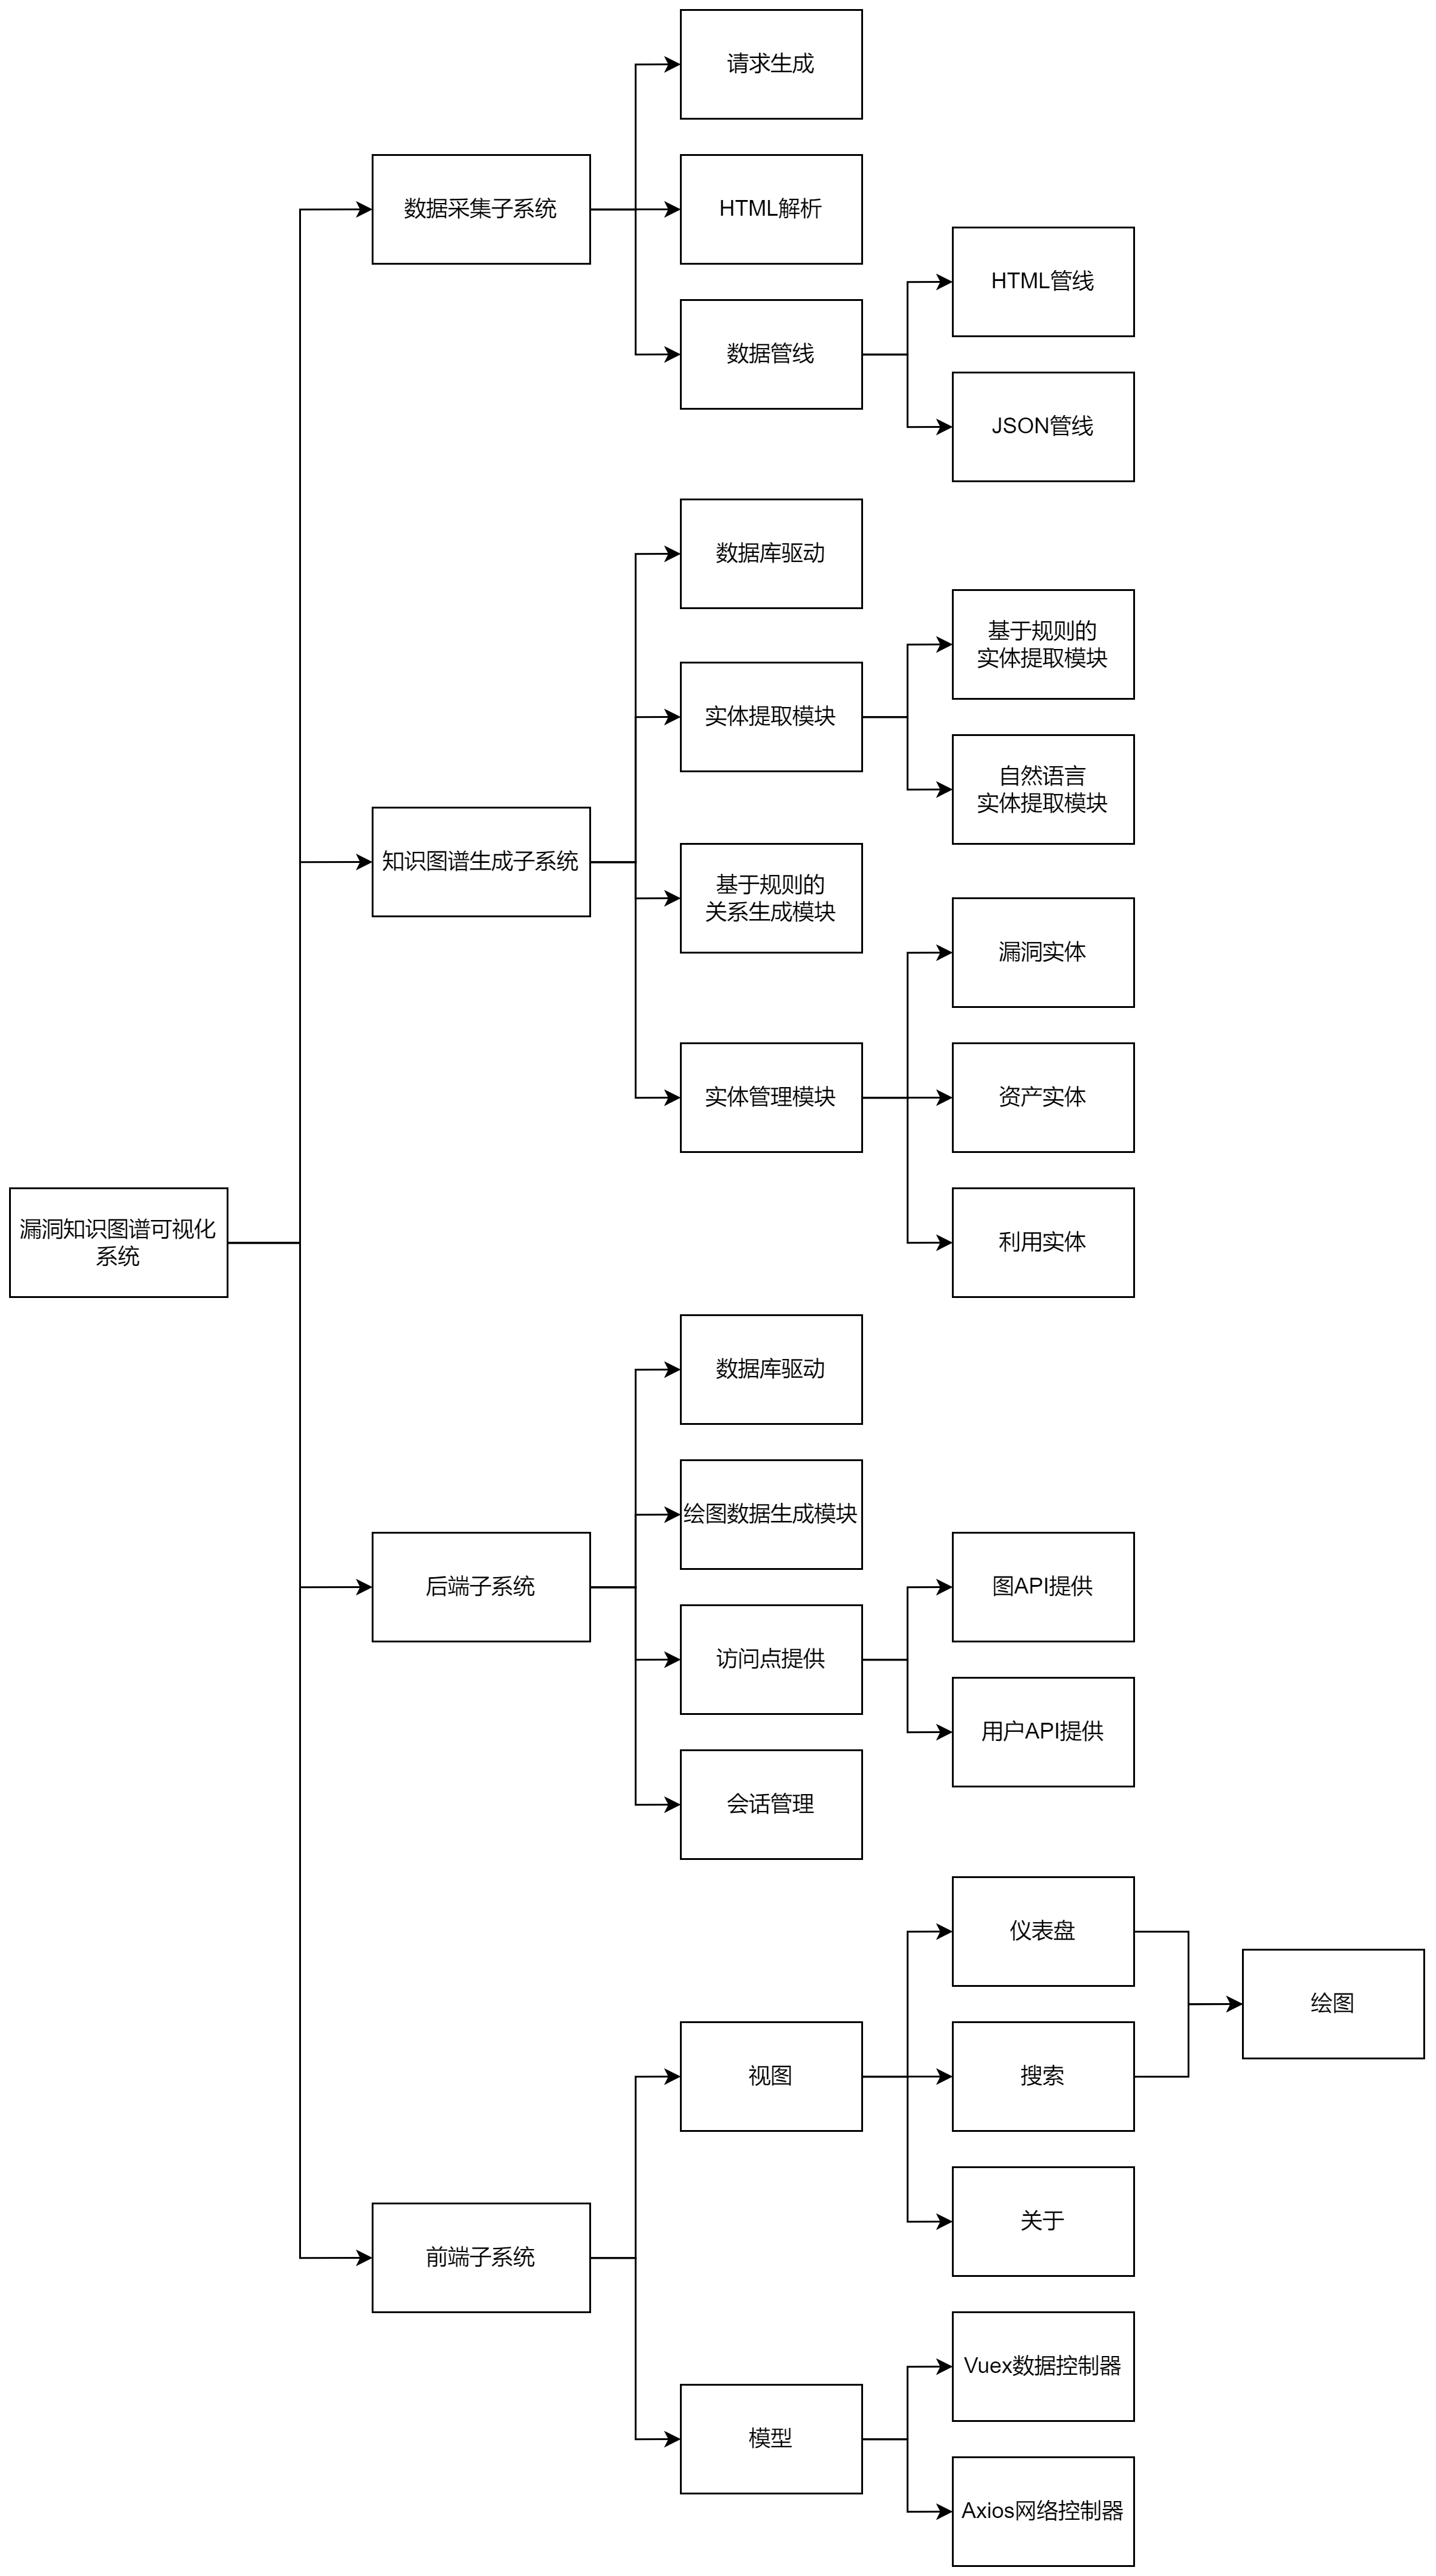
\includegraphics[height=0.95\textheight]{pictures/CyKG_OrgChart-中文.png}
	\caption{系统功能模块设计图}
	\label{CyKG_OrgChart}
\end{figure}

\subsection{数据采集子系统}

主要实现 Web 爬虫服务,包括请求生成器、异构数据解析器、异构数据管线三个模块。其中异构数据解析器包含包含 HTML 解析器、JSON 解析器、csv 解析器、gzip 解析器等。异构数据管线包含与异构数据解析器对应的各类数据管线。

请求生成器根据 csv 索引生成爬虫请求链接,交由 Scrapy Spider 进行并发爬虫。

异构数据解析器负责使用对应解析器解析 Spider 爬虫返回的网络数据,传递给异构数据管线。此外,异构数据解析器中的 HTML 解析器应用在一些网站的爬虫任务时,还会解析页面上包含“下一页”等元素的 <a> 标签,通过 yield 将其中 href URL 交给请求生成器,生成新的爬虫请求。

异构数据管线负责接收其对应的数据解析器传来的数据,提取其中需要的信息进行格式转换等处理,填充固定格式的 Python Dictionary,再调用持久化子系统中的数据库控制器对象,将请求原始数据与 Dictionary 分别存储至不同的 MongoDB 数据库集合(Collection)中持久化存储,形成原始数据,完成数据采集工作。

\subsection{知识图谱构建子系统}

主要实现知识图谱构建服务,包含实体生成模块、基于规则的关系生成模块、关系融合模块。

实体生成模块目前包含基于规则的实体生成子模块,未来可引入基于深度学习模型的自然语言实体生成子模块。实体生成模块从原始数据中提取资产类型、属性等信息,调用持久化子系统的数据库控制对象将结点存入 Neo4j 数据库。具体而言,分为漏洞结点生成、资产结点生成、利用代码结点生成三部分,分别生成漏洞结点、资产结点与资产家族结点、利用代码结点。

基于规则的关系生成模块利用不同类型实体间隐含的联系,在 Neo4j 数据库中匹配对应结点,在两个结点间生成对应的边,并为其添加属性。因知识图谱中预计将有一百万个结点,使用最细粒度将每个漏洞结点与每个资产结点连接将产生超过一亿条边,这对于本项目的性能要求而言是不现实的。因此,关系生成模块会使用前述步骤生成的资产家族结点,在漏洞结点与漏洞结点所包含的受影响资产列表中的每条正则匹配项所匹配到的资产对应的资产家族之间添加关系。为了维持该关系指向资产的语义准确,将匹配到的资产列表作为属性添加到该关系边之上。

关系融合模块://TODO

\subsection{后端服务子系统}

主要负责提供后端 Web API、对知识图谱的数据进行转换处理、调度各服务运行。包括绘图数据生成模块、Web API 访问点、APScheduler 调度模块。

Web API 访问点由 Flask 支持,使用 Flask 的 Blueprint 功能对注册在 RESTful API 根路径下的第一级 API 进行分组管理,实现模块化设计。在某个 Route 收到请求时,根据用户请求内容,将请求参数作为 CQL 参数,调用持久化层数据库控制对象对数据库进行操作,增删查改知识图谱中的结点和关系。若是可视化相关的 Route,则会对查询到的数据调用绘图数据生成模块进行转换。

绘图数据生成模块将存储在 Neo4j 数据库中的知识图谱数据转化为 ECharts 绘图库可以使用的数据格式。

APScheduler 调度模块://TODO

\subsection{前端子系统}

前端子系统负责管理用户运行时相关数据、通过 UI 向用户展示信息。使用 Vue.js 的 MVVM 架构,主要包含视图与模型两个组成部分。

视图包含控制台、可视化、搜索、关于四部分。控制台视图为用户提供知识图谱信息概览,包含列表形式的数据展现,以及统计图表形式的数据可视化。可视化视图是一个全屏视图,通过该视图用户可以一览知识图谱全貌。搜索视图只是用户在图谱中搜索感兴趣的内容,并将搜索结果以力引导图可视化的形式展示。关于视图展示本系统相关信息及用户指南。

模型主要包含 Vuex 数据控制器、Axios 网络控制器两部分。Vuex 数据控制器统一管理前端子系统的数据与状态,是前端子系统的“Single Source of Truth”,为视图的响应式显示提供数据源,还包含在前端对数据进行简单处理功能。Axios 网络控制器封装一个 httpCliet 对象,以及若干与后端通信的方法。Vuex 数据控制器可以调用 Axios 网络控制器,从后端获取数据,更新 Vuex Store 中的状态。

\subsection{数据库设计}

图\ref{CyKG_Entity-Mongo}所示为 MongoDB 数据模式图。//TODO

\buptfigure[height=0.5\textheight]{pictures/CyKG_Entity-Mongo.png}{MongoDB 数据模式图}{CyKG_Entity-Mongo}

图\ref{CyKG_Entity}所示为 Neo4j 数据模式图,同时也是知识图谱实体与关系模式图。

\buptfigure[height=0.5\textheight]{pictures/CyKG_Entity.png}{Neo4j 数据模式图}{CyKG_Entity}

\subsection{系统接口设计}

图\ref{api_table}展示了系统接口设计。
\begin{bupttable}{系统接口设计}{api_table}
	\begin{tabularx}{\textwidth}{llX}
		\toprule
		\textbf{类别} & \textbf{路径}         & \textbf{描述}                                         \\ \midrule
		              & /<path>               & 前端路由路径                                          \\ \cmidrule(l){2-3}
		              & /api/graph/           & 获取知识图谱统计信息                                  \\ \cmidrule(l){2-3}
		前端          & /api/graph/<limit>    & 获取与<limit>个漏洞结点相关联的结点或关系组成的子图谱 \\ \cmidrule(l){2-3}
		              & /api/search/<keyword> & 搜索与<keyword>关键字相关的结点或关系                 \\ \bottomrule %\midrule
	\end{tabularx}
\end{bupttable}

\section{系统详细设计}

\subsection{开发环境配置}

\begin{itemize}
	\item 操作系统:Ubuntu 20.04,Windows 11 Pro
	\item 数据采集子系统:Python 3.8,Scrapy 2.6
	\item 知识图谱构建子系统:Python 3.8,Ray 1.11.1,uuid 1.3
	\item 持久化子系统:Python 3.8,Py2neo 2021.2.3,Pymongo 3.12,Neo4j 4.4
	\item 后端服务子系统:Python 3.8,Flask 2.0,flask-cors 3.0
	\item 前端子系统:JavaScript ES6,Vue 2.6,Vuetify 2.6,ECharts 5.3.2,vue-axios 3.4,Vuex 3.4,Moment 2.29.3,Lodash 4.17.21
\end{itemize}

\subsection{各核心功能模块详细设计}

\subsubsection{类图}

\ref{CyKG_Class-DataCollection}

\buptfigure[width=\textwidth]{pictures/CyKG_Class-DataCollection.png}{数据采集子系统类图}{CyKG_Class-DataCollection}

\ref{CyKG_Class-KnowledgeGraphGeneration}

\buptfigure[width=\textwidth]{pictures/CyKG_Class-KnowledgeGraphGeneration.png}{知识图谱构建子系统类图}{CyKG_Class-KnowledgeGraphGeneration}

\ref{CyKG_Class-Backend}

\buptfigure[width=\textwidth]{pictures/CyKG_Class-Backend.png}{后端服务子系统类图}{CyKG_Class-Backend}

\subsubsection{功能时序图}

\ref{CyKG_Sequence-UserSequence}

\buptfigure[width=\textwidth]{pictures/CyKG_Sequence-UserSequence.png}{用户请求功能时序图}{CyKG_Sequence-UserSequence}

\chapter{系统实现}

\section{工具模块}

\subsection{根目录模块 bot{\_}root{\_}dir.py}

本模块位于项目根目录下。\lstinline[style = python]|get_bot_root_dir()| 方法使用 pathlib 的 \lstinline[style = python]|Path(__file__).parent| 方法获得项目根目录的路径,使得本项目内代码全部使用平台无关的相对路径,从而能在 Linux、macOS、Windows 等多种系统平台运行,保证可移植性。

本模块内包含许多路径相关的方法,如 \lstinline|get_source_data_dir(), get_cve_data_dir(), get_log_dir()| 等。这些方法接受字符串形式的路径参数,返回 \lstinline|Path| 对象。通过传入参数,控制系统生成的文件存放的位置,若目录不存在,则会自动创建所需目录。

本系统所有涉及文件系统的模块都依赖于此模块。

\subsection{日志模块 logger{\_}factory.py}

在 Python Logging 模块基础上重新实现了自定义的日志功能。具有 \lstinline|init_log_dir(), setup_logger(), mylogger(), loggers={}| 等方法和属性。

\lstinline|init_log_dir()| 接受字符串路径可选参数,初始化日志记录路径。若参数为空,则使用默认路径。

\lstinline|setup_logger(name, log_folder=None, lvl_file=None, lvl_stdout=None)| 是一个工厂函数,创建一个新的 Logger 对象,根据参数设置 \lstinline|FileHandler(), StreamHandler()|,支持自定义日志路径、文件名称和不同 Handler 使用不同记录等级。

\lstinline[style = python]|mylogger()| 实现 logger 对象的单例模式。利用 Python 模块引入为单例的特性,使得在同一模块内多次调用相同 \lstinline[style = python]|<name>| 的 \lstinline[style = python]|mylogger()| 会返回相同的 Logger 对象。当第一次调用 \lstinline|mylogger(<name>)| 时,会调用 \lstinline|setup_logger()| 创建一个新的 Logger 对象,并且将其保存在全局变量 loggers 字典内。之后调用同样的 \lstinline|mylogger(<name>)| 时,会根据 \lstinline|<name>| 从 loggers 字典查找对应的 Logger 对象并返回。

在一个模块内首次调用 \lstinline[style = python]|mylogger(<name>)| 会初始化日志,添加日志的文件控制器与标准输出控制器,并且设定输出日志文件位置,以“本模块名+当前时分秒”命名。后续再次调用 \lstinline[style = python]|mylogger(<name>).log()| 会使用首次创建的 logger 对象进行日志记录。

\subsection{环境配置文件 secret.py}

以 Python 变量的形式存储 MongoDB 与 Neo4j 数据库的用户名、密码、数据库名、连接 url 等信息,和一些私有 API 的密钥等信息。此文件被 \lstinline|.gitignore|,不会同步到远程仓库。

\section{数据采集子系统}

\subsection{Spider 模块实现}

每个 Spider 继承自\lstinline[style = python]|scrapy.Spider|类,重写了父类的 \lstinline[style = python]|__init__(), start_requests(),  parse()| 方法。

\subsubsection{{\_\_}init{\_\_}()}
% \subsubsection{\textunderscore \textunderscore init\textunderscore \textunderscore}

\lstinline[style = python]|__init__()| 方法完成 Spider 类的初始化工作。在调用父类的 \lstinline|super.__init__()| 方法之后,调用本系统基于 Python Logging 模块重新自定义封装的 \lstinline[style = python]|mylogger(<name>)| 函数初始化 logger。

\subsubsection{start{\_}requests()}
% \begin{lstlisting}[style = python]
% 	for x in range(101):
% 		print('fizz'[x%3*4:] + 'buzz'[x%5*4:] or x)
% 		print('Hello world!') yield scrapy.Request(url=url, callback=self.parse) yield scrapy.Request(url=url, callback=self.parse)
% \end{lstlisting}
\lstinline[style = python]|start_requests()| 方法描述发起请求的步骤。

对于需要 cve id 索引的 Spider 如 \lstinline[style = python]|CveDetailSpider(scrapy.Spider)|,使用 Pandas 库的 \lstinline[style = python]|read_csv()| 方法,设置 \verb|chunksize| 数值和 \verb|iterator=True|,分块迭代读取 csv 文件。对每一行 cve id,生成所需 url 并使用 \lstinline[style = python]|yield scrapy.Request(url=url, callback=self.parse)| 发出请求。

对于需要从爬取页面中获得下一页 url 的 Spider 如 \lstinline[style = python]|EdbSpider(scrapy.Spider)|,\linebreak \lstinline[style = python]|start_request()| 方法中仅指定初始页面发出请求,在解析收到的 response 时处理下一页面的链接,并发出请求。

对于采用 JavaScript 动态加载页面的站点如 exploit-db.com,使用将 playwright 无头浏览器与 Scrapy 框架集成的 scrapy-playwright 库,对爬取到的 HTML 页面及其 JavaScript 代码进行渲染,将渲染生成的 DOM 返回给 Spider 的 \lstinline[style = python]|parse()| 方法。

\subsubsection{parse()}

\lstinline[style = python]|parse()| 方法实现对请求返回数据的解析。

对于返回数据为 HTML 文档类型,使用 BeautifulSoup 库加载 DOM 进行解析。使用 \lstinline[style = python]|soup.select_one()| 方法配合 CSS 选择器提取所需标签的内容。对于需要在页面上查找下一请求 url 的站点,使用 \lstinline[style = python]|yield scrapy.Request()| 方法发出请求。将解析出的数据封装在 \lstinline[style = python]|scrapy.Item| 类中,使用 \lstinline[style = python]|yield item| 方法将数据传递给对应数据管线。

对于返回数据为 JSON 类型,使用 \lstinline[style = python]|response.json()| 获取返回数据,将其作为参数实例化 Item 对象,传递给 JSON 数据管线。

对于单个请求返回数据为 Gz 压缩的 xml 类型,使用工具模块 \lstinline[style = python]|gz.py| 的 \lstinline[style = python]|un_gz()| 方法解压文件得到 xml,并使用 lxml 模块的 \lstinline[style = python]|etree.iterparse(filepath, tag='')| 方法迭代遍历该 xml 文件,填充 item,最终调用持久化子系统的数据库控制对象提供的 \lstinline[style = python]|save_cpe()| 方法存储。

将以上代码段包裹在 Python 的 \lstinline|try...except...finally...| 语句内,使日志模块能正常 \lstinline|catch| 抛出的错误,并使程序不中断继续运行。

\subsection{Item Pipeline 模块实现}

每个 Pipeline 类实现一个 \lstinline[style = python]|process_item()| 方法,同时在 Spider 的 \lstinline[style = python]|custom_settings| 内设置对应的 Pipeline 类。Scrapy Engine 将 Spider 内 \lstinline[style = python]|yield item| 发送给 Pipeline 对象进行处理。

GzPipeline 负责处理压缩成 Gzip 格式的 cve 与 cpe xml 文件。将其解压并返回解压后文件的路径。

NvdPipeline 负责处理 NVD API 提供的 JSON,提取数据并调用持久化子系统的数据库控制对象提供的 \lstinline|save_nvd_src()| 方法存储原始数据,使用 \lstinline|save_nvd()| 方法存储处理过的数据。

其余 Pipeline 功能类似,根据爬取站点不同,实现有所不同。

\subsection{其他模块实现}

\begin{itemize}
	\item \lstinline|scrapy.cfg|:存放 Scrapy 项目设置选项,如默认设置文件、项目名称等。
	\item \lstinline|settings.py|:Python 变量形式存放 Scrapy 爬虫设置选项,如并发度、请求延时、User-Agent 等。
	\item \lstinline|crawl_runner| 目录:包含 \lstinline|crawl_cpe.py, crawl_nvd.py, crawl_edb.py| 等。使用\linebreak \lstinline|scrapy.cmdline.execute()| 方法运行爬虫程序。可以被调度模块调用实现全自动化爬虫。
\end{itemize}



\section{知识图谱构建子系统}

\section{持久化子系统}

\section{后端服务子系统}

\section{前端子系统}

\chapter{系统测试}

\section{测试环境}

\begin{itemize}
	\item CPU:AMD Ryzen ZEN3 架构 8C16T@4.8GHz
	\item RAM:16GB*2 DDR4@3600MT/s
	\item 存储:PCIe Gen 3 固态硬盘
	\item 操作系统:Ubuntu 20.04
\end{itemize}

\section{数据采集子系统测试}

图\ref{pictures/DB_Mongo-Overview.png}展示 MongoDB 数据库中的 Collections 概览。

\buptfigure[width=\textwidth]{pictures/DB_Mongo-Overview.png}{MongoDB Collections 概览}{pictures/DB_Mongo-Overview.png}

通过 Scrapy 爬虫 cve.mitre.org,获得约 23 万条 cve id 数据,经筛选清洗获得约 16 万条有效 cve id 信息,如图\ref{pictures/DB_Cve.png}所示。

\buptfigure[width=\textwidth]{pictures/DB_Cve.png}{cve id 索引 csv 数据}{pictures/DB_Cve.png}

爬取 cpe.mitre.org 定期发布的官方 cpe 信息文件,使用 lxml 库解析,经筛选清洗获得约 90 万条有效 cpe 资产信息 JSON 数据。其中包含用于识别的 cpe23uri、cpe 资产名称、参考资料链接等属性,如图\ref{pictures/DB_Cpe.png}所示。

\buptfigure[height=0.45\textheight]{pictures/DB_Cpe.png}{cpe 资产 JSON 数据}{pictures/DB_Cpe.png}

爬取 cvedetails.com,获得约 16 万个 HTML 页面,清洗整理获得超 400 万个 cve 漏洞与资产相关属性 JSON 数据,如图\ref{pictures/DB_Cvedetails.png}所示。

\buptfigure[height=0.45\textheight]{pictures/DB_Cvedetails.png}{cvedetails.com JSON 数据}{pictures/DB_Cvedetails.png}

通过 nvd.nist.gov JSON API 数据接口,获得约 16 万条 JSON 数据,包含漏洞名称与简介、漏洞条目发布日期、漏洞条目更新日期、CVSS 风险评级、参考资料、受影响资产的 cpe23uri 匹配正则表达式等信息,如图\ref{pictures/DB_Nvd.png}所示。

\buptfigure[height=0.45\textheight]{pictures/DB_Nvd.png}{nvd.nist.gov JSON 数据}{pictures/DB_Nvd.png}

爬取 exploit-db.com,获得约 5 万个 HTML 页面,包含漏洞利用代码、作者、发布时间、适用平台、利用类型、利用 cve id 等信息,清洗处理为 JSON 格式数据,如图\ref{pictures/DB_edb_json.png}所示。

\buptfigure[height=0.45\textheight]{pictures/DB_edb_json.png}{exploit-db.com JSON 数据}{pictures/DB_edb_json.png}

\section{知识图谱构建子系统测试}

\subsection{结点生成}

使用 Ray 库提供的 @Ray.remote 装饰器与 ray.get() 方法,将全部漏洞数据根据并行度参数进行分割,开辟多进程对分块漏洞数据进行生成结点操作。

开辟 32 个进程生成漏洞结点、资产结点、资产家族结点、漏洞利用结点,总计约 120 万个结点。系统耗时约 5 分钟,如图\ref{pictures/Gen_Nodes.png}与图\ref{pictures/DB_Nodes.png}所示。

\buptfigure[width=\textwidth]{pictures/Gen_Nodes.png}{结点生成模块运行日志}{pictures/Gen_Nodes.png}

\buptfigure[width=0.5\textwidth]{pictures/DB_Nodes.png}{数据库查询结点数量}{pictures/DB_Nodes.png}

\subsection{关系生成}

使用 Ray 库提供的 @Ray.remote 装饰器与 ray.get() 方法,将全部漏洞数据根据并行度参数进行分割,开辟多进程对分块漏洞数据进行生成操作。

开辟 32 个进程生成“资产$-[$具有$]->$漏洞,漏洞$-[$影响$]->$资产;资产$-[$是子级$]->$资产家族,资产家族$-[$是父级$]->$资产;利用代码$-[$攻击$]->$资产,资产$-[$被攻击$]->$利用代码;利用代码$-[$利用$]->$漏洞,漏洞$-[$被利用$]->$漏洞代码”等关系,由于资产关系生成涉及正则匹配运算,无法有效利用数据库索引,且 CPU 性能消耗较大,因此生成时间较长。对总计约 120 万个结点共生成约 45 万条边(更多详细信息存储在边属性中),耗时约 1 小时 50 分钟,如图\ref{pictures/Gen_Rels.png}与图\ref{pictures/DB_Rels.png}所示。

\buptfigure[width=\textwidth]{pictures/Gen_Rels.png}{关系生成模块运行日志}{pictures/Gen_Rels.png}

\buptfigure[width=\textwidth]{pictures/DB_Rels.png}{数据库查询关系数量}{pictures/DB_Rels.png}

\subsection{关系融合}

本系统设计上,结构化数据生成的漏洞实体具有 cve id 属性作为唯一标识;资产实体具有 cpe23uri 属性作为唯一标识;漏洞利用代码实体具有 edb-id 属性作为唯一标识。且在数据库控制器对象的方法中,使用 MERGE 等 CQL 子句保证不会向数据库插入重复的实体或属性。因此当前知识图谱内并不会出现语义相同的不同实体或关系。

关系融合模块作为适配使用深度学习模型进行命名实体识别结点生成与关系抽取方案的模块,当前仅在系统数据加工管线中留有接口,以备未来扩展需要。因此暂不作测试。

\section{数据库子系统与后端服务子系统测试}

\subsection{/api/graph/}

向运行在 localhost 上的后端服务子系统发送 /api/graph/ 请求,获取当前知识图谱基础统计信息。后端返回各类资产数量统计、各类漏洞数量统计、各类代码利用数量统计等信息,如图\ref{pictures/Backend_api-graph-content.png}所示。

\buptfigure[height=0.4\textheight]{pictures/Backend_api-graph-content.png}{/api/graph/ 请求响应数据}{pictures/Backend_api-graph-content.png}

耗时约 200 毫秒,如图\ref{pictures/Backend_api-graph.png}所示。

\buptfigure[height=0.4\textheight]{pictures/Backend_api-graph.png}{/api/graph/ 请求响应摘要}{pictures/Backend_api-graph.png}

\subsection{/api/graph/<limit>}

向运行在 localhost 上的后端服务子系统发送 /api/graph/100 请求,获取当前知识图谱的 100 个漏洞结点以及与其相关的资产、利用代码结点、关系等信息,用于可视化。后端返回经绘图数据生成模块处理的绘图数据,包含分类、结点、关系三个数组,如图\ref{pictures/Backend_api-graph-100-content.png}所示。

\buptfigure[height=0.4\textheight]{pictures/Backend_api-graph-100-content.png}{/api/graph/100 请求响应数据}{pictures/Backend_api-graph-100-content.png}

耗时约 640 毫秒,如图\ref{pictures/Backend_api-graph-100.png}所示。

\buptfigure[height=0.4\textheight]{pictures/Backend_api-graph-100.png}{/api/graph/100 请求响应摘要}{pictures/Backend_api-graph-100.png}

\section{前端子系统测试}

\subsection{控制台视图}

图\ref{pictures/Vis_Dashboard_Info.png}所示为控制台概览。从 localhost 后端 /api/graph/ 端口加载数据,实际返回,根据瀑布流图可看出,通过刷新页面冷加载控制台界面及各种网络请求耗时约 850ms,且加载过程中可视化图表有加载指示器提示正在加载、数据列表有默认数据“0”填充而非显示空白,用户体验较好。如图\ref{pictures/Dashboard_Waterfall.png}所示。

\buptfigure[width=\textwidth]{pictures/Vis_Dashboard_Info.png}{控制台视图预览}{pictures/Vis_Dashboard_Info.png}

\buptfigure[width=\textwidth]{pictures/Dashboard_Waterfall.png}{控制台视图加载请求瀑布流}{pictures/Dashboard_Waterfall.png}

\subsection{可视化视图}

图\ref{pictures/Vis_Full.png}所示为知识图谱概览。从 localhost 后端 /api/graph/100 端口加载数据,实际返回 1070 个结点、2035 条关系边,根据瀑布流图可看出,通过刷新页面冷加载可视化力引导图耗时约 1300ms,且加载过程中有加载指示器提示正在加载,用户体验较好。如图\ref{pictures/Vis_Waterfall.png}所示。

\buptfigure[width=\textwidth]{pictures/Vis_Full.png}{可视化视图概览}{pictures/Vis_Full.png}

\buptfigure[width=\textwidth]{pictures/Vis_Waterfall.png}{可视化视图加载请求瀑布流}{pictures/Vis_Waterfall.png}

图\ref{pictures/Vis_Detail.png}所示为知识图谱细节图。力引导图为有向图,因此结点间的无向边使用两条有向边表示。图中蓝色结点为漏洞结点,绿色结点为资产家族结点,红色结点为受影响资产结点。可以看到,通过将漏洞所影响的大量资产关系替换成漏洞到资产家族的一个关系,大幅简化了图的结构,在使视觉观感清晰的同时,将鼠标移至漏洞至资产家族的边上可显示受该漏洞影响的所有资产,保证图谱数据的详细精确。

\buptfigure[width=\textwidth]{pictures/Vis_Detail.png}{可视化视图细节}{pictures/Vis_Detail.png}

图\ref{pictures/Vis_Info.png}所示为当鼠标移动至或触摸图中元素,包括各类结点和各类关系,会显示 tooltip 指示,展现当前高亮元素的详细信息。

\buptfigure[width=\textwidth]{pictures/Vis_Info.png}{可视化视图 tooltip 展示详细信息}{pictures/Vis_Info.png}

\subsection{搜索视图}

图\ref{}所示为搜索视图。搜索视图提供一个悬浮搜索框,允许用户对知识图谱进行精确查询。输入查询关键字并按下回车,后端服务将搜索整个知识图谱查找关键字相关信息,并以绘图数据形式将结果返回前端。前端随即调用 ECharts 可视化库展示数据。

% \buptfigure[width=\textwidth]{pictures/Vis_Info.png}{可视化视图 tooltip 展示详细信息}{pictures/Vis_Info.png}

\subsection{关于视图}

图\ref{}所示为关于视图。关于视图清晰地展示了本系统名称、功能、作者、使用指南等信息。

% \buptfigure[width=\textwidth]{pictures/Vis_Info.png}{可视化视图 tooltip 展示详细信息}{pictures/Vis_Info.png}

\chapter{结束语}

%%%%%%%%%%%%%%%%%%%%%%% Main Area ENDs Here %%%%%%%%%%%%%%%%%%%%%%%%
%\let\cleardoublepage=\cleardoublepagebak

\begin{nopagenumber}
	% Reference
	\clearpage\phantomsection\addcontentsline{toc}{chapter}{参考文献}
	\bibliographystyle{buptbachelor}
	\refbodyfont{\bibliography{ref}}

	% Thanks to page
	\clearpage
	\chapter{致\qquad{}谢}
	\normalsize\thankwords

	% Appendix
	\setcounter{figure}{0}
	\renewcommand{\thefigure}{~附-\arabic{figure}~}
	\setcounter{equation}{0}
	\renewcommand{\theequation}{~附-\arabic{equation}~}
	\setcounter{table}{0}
	\renewcommand{\thetable}{~附-\arabic{table}~}
	\setcounter{lstlisting}{0}
	\makeatletter
	\renewcommand \thelstlisting
	{附-\@arabic\c@lstlisting}
	\makeatother


	\chapter*{附\qquad{}录}
	\phantomsection\addcontentsline{toc}{chapter}{附\qquad{}录}

	\phantomsection
	\addcontentsline{toc}{section}{附录1\quad{}缩略语表}
	\section*{附录1\quad{}缩略语表}

	\begin{bupttable}{基于浏览者行为的特征}{crowdwisdom2}
		\begin{tabular}{l|l|l}
			\hline \textbf{特征} & \textbf{描述}  & \textbf{形式与理论范围} \\
			\hline 点赞量        & 微博的点赞数量 & 数值,$\mathbb{N}$      \\
			\hline 评论量        & 微博的评论数量 & 数值,$\mathbb{N}$      \\
			\hline 转发量        & 微博的转发数量 & 数值,$\mathbb{N}$      \\
			\hline
		\end{tabular}
	\end{bupttable}

	\begin{bupttable}{基于浏览者行为的复杂特征}{complexcrowdwisdom2}
		\begin{tabular}{l|l|l|l}
			\hline
			\multicolumn{1}{c|}{\multirow{2}{*}{\textbf{类别}}} & \multicolumn{1}{c|}{\multirow{2}{*}{\textbf{特征}}} & \multicolumn{2}{c}{\textbf{不知道叫什么的表头}}                                               \\
			\cline{3-4}
			                                                    &                                                     & \multicolumn{1}{c|}{\textbf{描述}}              & \multicolumn{1}{c}{\textbf{形式与理论范围}} \\
			\hline
			\multirow{3}{*}{正常互动}                           & 点赞量                                              & 微博的点赞数量                                  & 数值,$\mathbb{N}$                          \\
			\cline{2-4}
			                                                    & 评论量                                              & 微博的评论数量                                  & 数值,$\mathbb{N}$                          \\
			\cline{2-4}
			                                                    & 转发量                                              & 微博的转发数量                                  & 数值,$\mathbb{N}$                          \\
			\hline
			非正常互动                                          & 羡慕量                                              & 微博的羡慕数量                                  & 数值,$\mathbb{N}$                          \\
			\hline
		\end{tabular}
	\end{bupttable}
	\buptfigure[width=0.15\textheight]{pictures/autoencoder}{自编码器结构}{autoencoder}

	\begin{lstlisting}[language=Python, caption=减法, label=minus, tabsize=2]  
def minusFunc(a, b):
	return a - b 
\end{lstlisting}

	\begin{equation}
		\label{PCA_goal}
		\begin{aligned}
			\max_{\substack{\bm{W}}} & tr(\bm{W}^\mathrm{T}\bm{X}\bm{X}^ \mathrm{T}\bm{W})
		\end{aligned}
	\end{equation}

	\clearpage
	\phantomsection
	\addcontentsline{toc}{section}{附录2\quad{}数学符号}
	\section*{附录2\quad{}数学符号}
	\begin{center}
		\begin{tabular}{ccc}
			\multicolumn{2}{c}{\textbf{数和数组}}                          \\
			\\
			$a$                 & 标量(整数或实数)                       \\
			$\bm{a}$            & 向量                                     \\
			$dim()$             & 向量的维数                               \\
			$\bm{A}$            & 矩阵                                     \\
			$\bm{A}^\mathrm{T}$ & 矩阵$\textbf{A}$的转置                   \\
			$\bm{I}$            & 单位矩阵(维度依据上下文而定)           \\
			$diag(\bm{a})$      & 对角方阵,其中对角元素由向量$\bm{a}$确定 \\
		\end{tabular}
	\end{center}

	\newpage\backmatter

	% Translated Article
	\blankmatter
	\thispagestyle{empty}
	\begin{center}
		% 原文第一页,PDF缩放比例为0.95,可以自行调整
		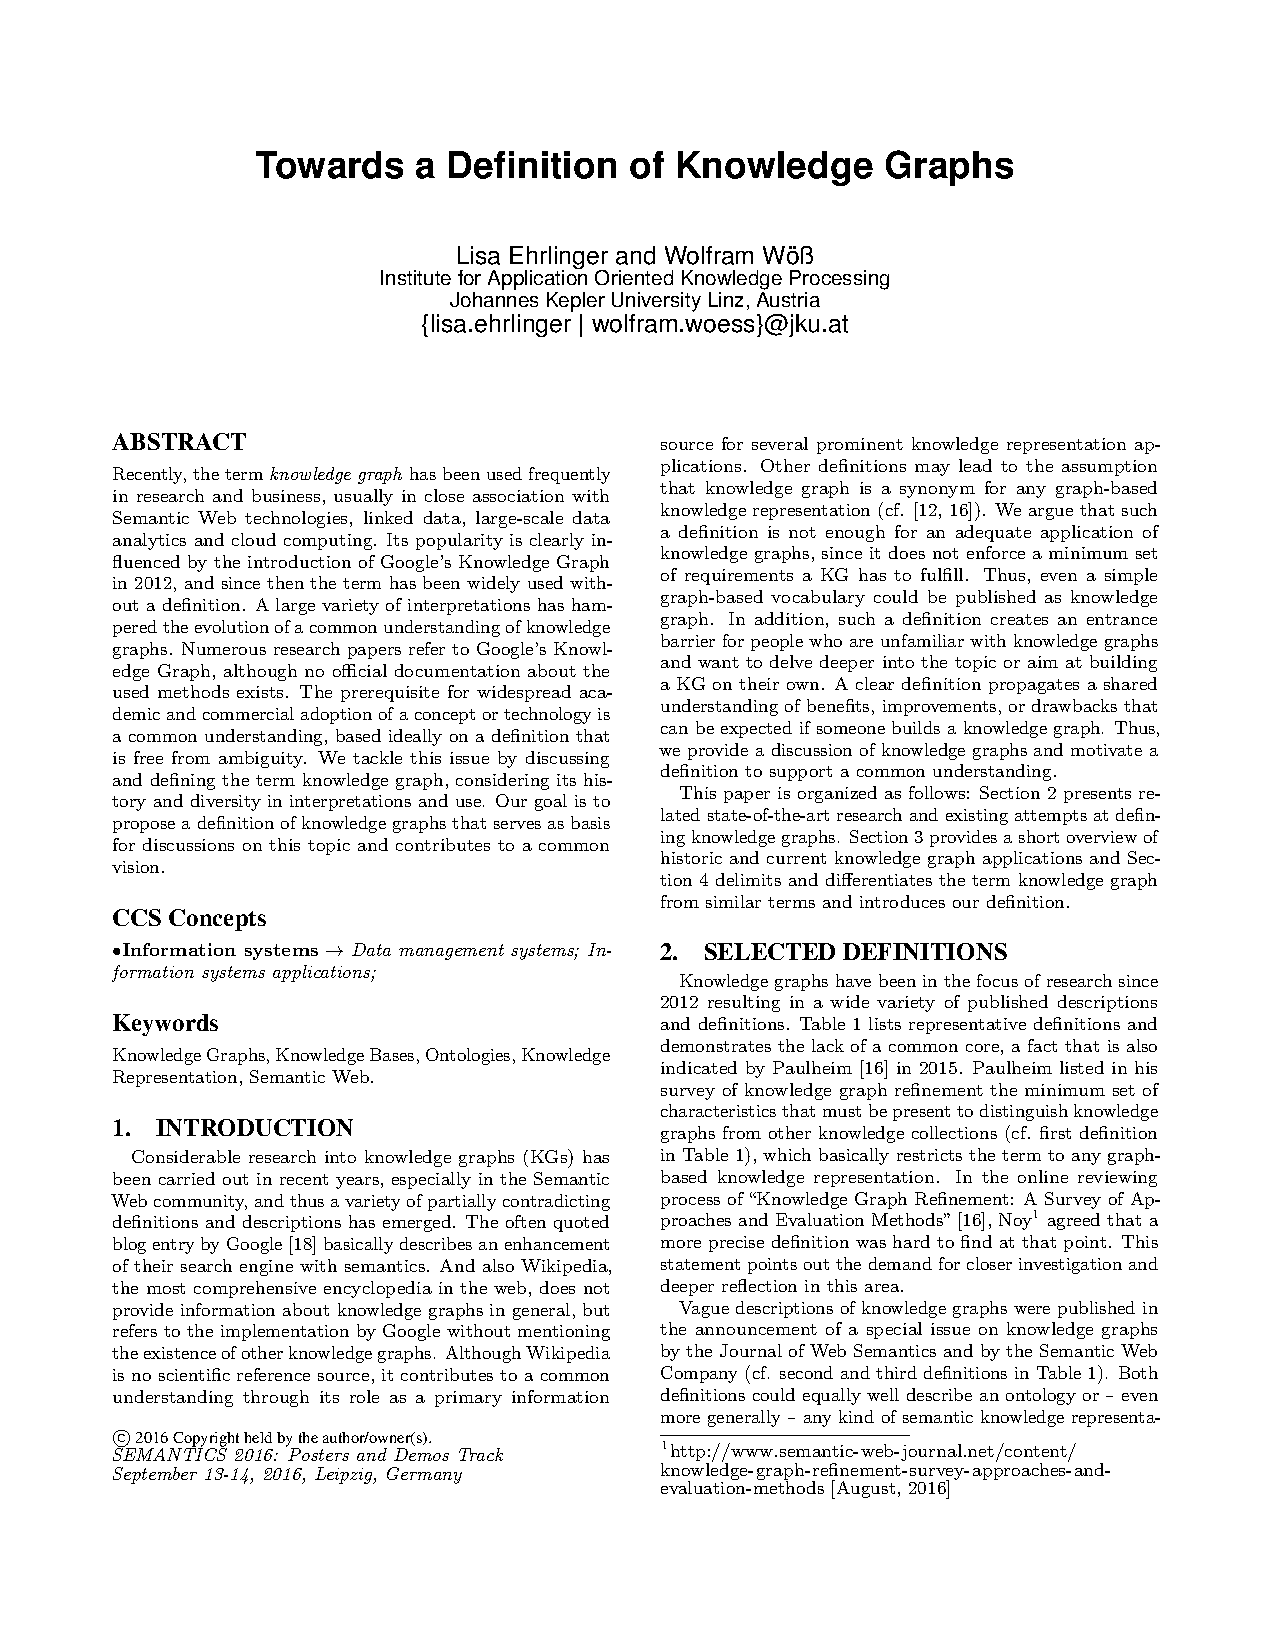
\includepdf[pages=1, scale=0.95, pagecommand=\heiti\sanhao{外\quad{}文\quad{}原\quad{}文}]{docs/translation.pdf}
		% 原文剩余部分
		\includepdf[pages=2-, scale=0.95, pagecommand={}]{docs/translation.pdf}
	\end{center}

	% Translation
	\setcounter{chapter}{0}
	\renewcommand{\thefigure}{~外\arabic{chapter}-\arabic{figure}~}
	\renewcommand{\theequation}{~外\arabic{chapter}-\arabic{equation}~}
	\renewcommand{\thetable}{~外\arabic{chapter}-\arabic{table}~}

	\begin{center}
		\translationtitlefont{外\quad{}文\quad{}译\quad{}文}
	\end{center}
	\vspace{8mm}
	\thispagestyle{empty}


	\begin{center}
		\sanhao\heiti\textbf{真假新闻的在线传播}

		\xiaosihao\songti{Soroush Vosoughi, Deb Roy, Sinan Aral}

		\xiaosihao\songti{麻省理工学院}
	\end{center}

	\songti{}
	\begingroup % 限制两个let语句的作用范围在外文译文部分
	\let\clearpage\relax
	\let\cleardoublepage\relax

	%以下是排版示例,在这里为了使章节编号不出现在目录中,使用了无编号的样式,代价是这些数字都要自己书写。

	\chapter*{第一章\quad{}概述}
	%每一个chapter后记得以下两行
	\newtranschapter

	\section*{1.1\quad{}概述}
	决策、合作、通信和市场领域的基础理论全都将对真实或准确度的概念化作为几乎一切人类努力的核心。然而,不论是真实信息还是虚假信息都会于在线媒体上迅速传播。定义什么是真、什么是假成了一种常见的政治策略,而不是基于一些各方同意的事实的争论。我们的经济也难免遭受虚假信息传播的影响。虚假流言会影响股价和大规模投资的动向,例如,在一条声称巴拉克·奥巴马在爆炸中受伤的推文发布后,股市市值蒸发了1300亿美元。的确,从自然灾害到恐怖袭击,我们对一切事情的反应都受到了扰乱。

	新的社交网络技术在使信息的传播速度变快和规模变大的同时,也便利了不实信息(即不准确或有误导性的信息)的传播。然而,尽管我们对信息和新闻的获取越来越多地收到这些新技术的引导,但我们仍然对他们在虚假信息传播上的作用知之甚少。尽管媒体对假新闻传播的轶事分析给予了相当多的关注,但仍然几乎没有针对不实信息扩散或其发布源头的大规模实证调查。目前,虚假信息传播的研究仅仅局限于小的、局部的样本的分析上,而这些分析忽略了两个最重要的科学问题:真实信息和虚假信息的传播有什么不同?哪些人类判断中的因素可以解释这些不同?

	\begin{equation}
		\label{PCA_goal_appx1}
		\begin{aligned}
			\max_{\substack{\bm{W}}} & tr(\bm{W}^\mathrm{T}\bm{X}\bm{X}^ \mathrm{T}\bm{W})
		\end{aligned}
	\end{equation}

	我只是为了把第二章挤到下一页而凑的字。我只是为了把第二章挤到下一页而凑的字。我只是为了把第二章挤到下一页而凑的字。我只是为了把第二章挤到下一页而凑的字。我只是为了把第二章挤到下一页而凑的字。我只是为了把第二章挤到下一页而凑的字。我只是为了把第二章挤到下一页而凑的字。我只是为了把第二章挤到下一页而凑的字。我只是为了把第二章挤到下一页而凑的字。我只是为了把第二章挤到下一页而凑的字。我只是为了把第二章挤到下一页而凑的字。我只是为了把第二章挤到下一页而凑的字。我只是为了把第二章挤到下一页而凑的字s。我只是为了把第二章挤到下一页而凑的字。我只是为了把第二章挤到下一页而凑的字。我只是为了把第二章挤到下一页而凑的字。我只是为了把第二章挤到下一页而凑的字。我只是为了把第二章挤到下一页而凑的字。我只是为了把第二章挤到下一页而凑的字。我只是为了把第二章挤到下一页而凑的字。我只是为了把第二章挤到下一页而凑的字。我只是为了把第二章挤到下一页而凑的字。我只是为了把第二章挤到下一页而凑的字。我只是为了把第二章挤到下一页而凑的字。

	\newpage %每一章需要另起一页,为了灵活,我没有把它固定在样式中,你可以根据需求添加分页符
	\chapter*{第二章\quad{}我也不知道是什么}
	\newtranschapter

	新的社交网络技术在使信息的传播速度变快和规模变大的同时,也便利了不实信息(即不准确或有误导性的信息)的传播。然而,尽管我们对信息和新闻的获取越来越多地收到这些新技术的引导,但我们仍然对他们在虚假信息传播上的作用知之甚少。尽管媒体对假新闻传播的轶事分析给予了相当多的关注,但仍然几乎没有针对不实信息扩散或其发布源头的大规模实证调查。目前,虚假信息传播的研究仅仅局限于小的、局部的样本的分析上,而这些分析忽略了两个最重要的科学问题:真实信息和虚假信息的传播有什么不同?哪些人类判断中的因素可以解释这些不同?

	新的社交网络技术在使信息的传播速度变快和规模变大的同时,也便利了不实信息(即不准确或有误导性的信息)的传播。然而,尽管我们对信息和新闻的获取越来越多地收到这些新技术的引导,但我们仍然对他们在虚假信息传播上的作用知之甚少。尽管媒体对假新闻传播的轶事分析给予了相当多的关注,但仍然几乎没有针对不实信息扩散或其发布源头的大规模实证调查。目前,虚假信息传播的研究仅仅局限于小的、局部的样本的分析上,而这些分析忽略了两个最重要的科学问题:真实信息和虚假信息的传播有什么不同?哪些人类判断中的因素可以解释这些不同?

	新的社交网络技术在使信息的传播速度变快和规模变大的同时,也便利了不实信息(即不准确或有误导性的信息)的传播。然而,尽管我们对信息和新闻的获取越来越多地收到这些新技术的引导,但我们仍然对他们在虚假信息传播上的作用知之甚少。尽管媒体对假新闻传播的轶事分析给予了相当多的关注,但仍然几乎没有针对不实信息扩散或其发布源头的大规模实证调查。目前,虚假信息传播的研究仅仅局限于小的、局部的样本的分析上,而这些分析忽略了两个最重要的科学问题:真实信息和虚假信息的传播有什么不同?哪些人类判断中的因素可以解释这些不同?

	\begin{equation}
		\label{PCA_goal_appx2}
		\begin{aligned}
			\max_{\substack{\bm{W}}} & tr(\bm{W}^\mathrm{T}\bm{X}\bm{X}^ \mathrm{T}\bm{W})
		\end{aligned}
	\end{equation}

	新的社交网络技术在使信息的传播速度变快和规模变大的同时,也便利了不实信息(即不准确或有误导性的信息)的传播。然而,尽管我们对信息和新闻的获取越来越多地收到这些新技术的引导,但我们仍然对他们在虚假信息传播上的作用知之甚少。尽管媒体对假新闻传播的轶事分析给予了相当多的关注,但仍然几乎没有针对不实信息扩散或其发布源头的大规模实证调查。目前,虚假信息传播的研究仅仅局限于小的、局部的样本的分析上,而这些分析忽略了两个最重要的科学问题:真实信息和虚假信息的传播有什么不同?哪些人类判断中的因素可以解释这些不同?

	新的社交网络技术在使信息的传播速度变快和规模变大的同时,也便利了不实信息(即不准确或有误导性的信息)的传播。然而,尽管我们对信息和新闻的获取越来越多地收到这些新技术的引导,但我们仍然对他们在虚假信息传播上的作用知之甚少。尽管媒体对假新闻传播的轶事分析给予了相当多的关注,但仍然几乎没有针对不实信息扩散或其发布源头的大规模实证调查。目前,虚假信息传播的研究仅仅局限于小的、局部的样本的分析上,而这些分析忽略了两个最重要的科学问题:真实信息和虚假信息的传播有什么不同?哪些人类判断中的因素可以解释这些不同?

	新的社交网络技术在使信息的传播速度变快和规模变大的同时,也便利了不实信息(即不准确或有误导性的信息)的传播。然而,尽管我们对信息和新闻的获取越来越多地收到这些新技术的引导,但我们仍然对他们在虚假信息传播上的作用知之甚少。尽管媒体对假新闻传播的轶事分析给予了相当多的关注,但仍然几乎没有针对不实信息扩散或其发布源头的大规模实证调查。目前,虚假信息传播的研究仅仅局限于小的、局部的样本的分析上,而这些分析忽略了两个最重要的科学问题:真实信息和虚假信息的传播有什么不同?哪些人类判断中的因素可以解释这些不同?

	\endgroup
\end{nopagenumber}

% 开题报告
\blankmatter

\includepdf[pages=-]{docs/openingReport.pdf}


% 中期检查表
\blankmatter

\includepdf[pages=-]{docs/interimReport.pdf}


\end{document}
